\section{Elément d'optique}

\subsection{Dioptre plan}

\subsubsection{Rayon linéaire}

Le dioptre est une surface qui sépare deux milieux transparents homogènes et isotropes ayant un indice de réfraction différent.
Pour connaître l'indice de réfraction le plus important, il suffit de déterminer quel est l'angle 
le plus grand entre l'angle d'incidence et l'angle de réfraction. Puis, avec la loi de \textbf{Snell-Descartes}, il est 
possible de retrouver l'indice de réfraction du deuxième milieu ($n_2$) : 

\begin{framed}
$$ n_2.sin(i_2) = n_1.sin(i_1) \Rightarrow n_2 = \frac{n1*sin(i_1)}{sin(i_2)} $$
\end{framed}

A partir de cette formule, on peut voir que si l'angle i1 est plus grand que l'angle i2, alors l'indice de réfraction le plus petit
est n1. \newline

%Si nous prenons les données de la simulation disponible sur le site du master IVI, en prenant comme indice de réfraction
%1 pour le milieu 1, nous obtenons le résultat suivant :

%\begin{framed}
%$$ n_2 = \frac{1*sin(41)}{sin(19)}=2,02$$
%\end{framed}

\subsubsection{Source ponctuelle}

Un système optique est dit stigmate s'il dévie les rayons d'un point source de telle sorte qu'il soit à nouveau concourant en 
un point en sortant du système.\newline

La simulation 2 que nous étudions ne possède pas un système optique stigmate car si on prolonge les rayons du milieu 2 dans le milieu
1, ceux-ci ne convergent plus en un seul point. Il semble que plus la source de lumière est éloignée et moins elle est étalée, plus 
le dioptre adopte un comportement stigmate. 
Lorsque le système se rapproche de ce comportement, on peut dire que l'image est virtuelle car 
le point de ``convergence'' des rayons lumineux se situe derrière le système optique.\newline

\begin{figure}[H]
      \center
      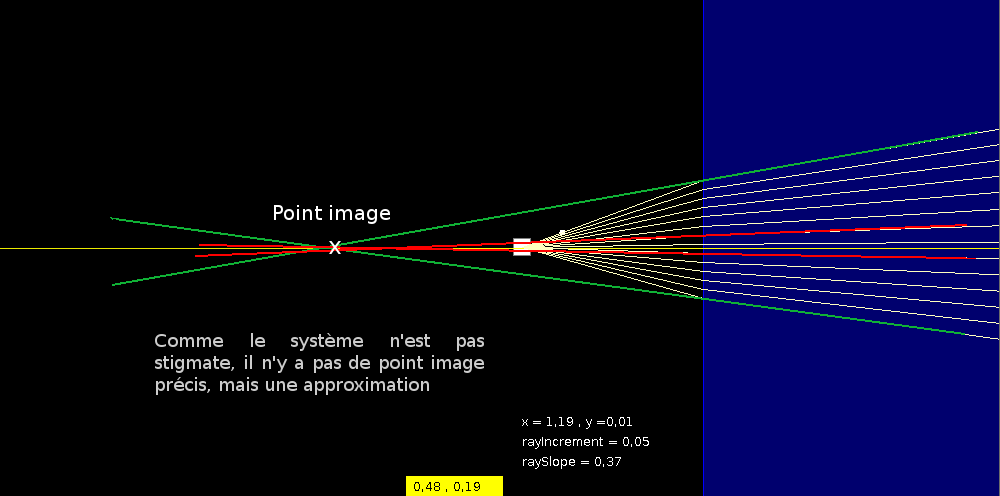
\includegraphics[width=14cm]{ressources/tp1/source_ponctuelle1.png}
      \caption{Source ponctuelle}
\end{figure}

La réaction de ce système fait qu'un observateur qui est à droite du dioptre de la simulation, verra l'objet plus 
éloigné qu'il ne l'est vraiment. Comme le système n'est pas stigmate, l'image aura une légère distorsion aux yeux 
de l'observateur. Ces phénomènes sont expliqués par le fait que si on prolonge les rayons du milieu 2 dans le milieu 1,
l'ensemble des prolongements coupe l'axe optique\footnote{la normale du dioptre} derrière l'objet (source de lumière) et 
ces prolongements ne sont pas concourants.\newline

Lorsque l'on inverse les deux milieux, on voit que les angles et les propriétés du dioptre sont inversés. Le système reste donc astigmate 
et l'image est toujours virtuelle.
Pour l'observateur se trouvant à droite du système optique, l'objet apparaîtra plus gros, et il semblera plus proche toujours avec une distorsion.
%ajout de l'image de la simulation

\subsection{Réflexion totale}

La réflexion totale est un phénomène qui fait qu'à partir d'un certain angle d'incidence un rayon lumineux ne quitte plus son milieu.
Nous allons voir ce phénomène dans la seconde simulation qui représente une plaque à faces parallèles.\\

Lorsque la source lumineuse est dans le milieu un, on voit qu'il y a un léger décalage entre les rayons entrants et sortants de la plaque.
Cependant, ces rayons restent parallèles entre eux.
Les effets des deux dioptres s'annulent étant donné que le milieu à gauche du premier dioptre est le même que le milieu à 
droite du second dioptre.\newline

On constate que lorsque la source lumineuse se retrouve entre les deux dioptres, les rayons restents à l'intérieur de la plaque.
Cet effet est annulé lorsque l'angle d'incidence est inférieur ou égale à 0,47 radian soit environ 27 degrès.
Cette limite nous permet de déterminer l'indice de réfraction du milieu situé entre les deux dioptres 
grâce au calcul suivant : 

\begin{framed}
$$ n_2 = \frac{1 * sin(27)}{sin(79)} = 0,46 $$
\end{framed}

\begin{figure}[H]
      \center
      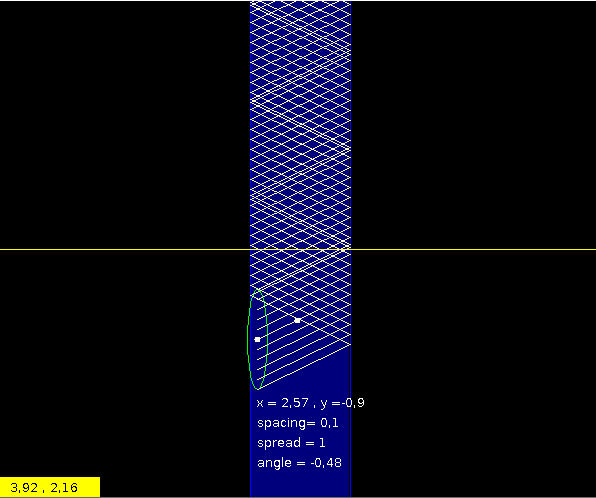
\includegraphics[width=10cm]{ressources/tp1/reflexion_totale.png}
      \caption{Illustration de l'effet FTIR avec un angle de 28 degrès}
\end{figure}

A partir de cet angle, il est possible de retrouver le demi-angle de la diode. En effet, le dioptre à la surface 
du plexiglas et les dioptres sur les arêtes du plexiglas sont différents. Il faut donc faire correspondre l’angle trouvé 
auparavant avec l’angle de réfraction de la diode placée en face de l’arête du plexiglas, c’est le demi-angle de cette 
diode qui est réfracté en passant par l’arête du plexiglas, puis se réfléchit sur la surface du plexiglas, à l'intérieur 
de celui-ci. Ce phénomène est appelé réflexion totale ou FTIR\footnote{Frustrated Total Internal Reflection}.

%Ce résultat permet de déterminer le demi-angle maximal(noté x) d'émission d'une LED\footnote{diode électroluminescente} permettant d'éclairer 
%le bord de la plaque de plexiglas afin d'obtenir un effet FTIR en effectuant le calcule suivant : \newline


%\begin{framed}
%Soit $i_3 = i_2$ de l'ancien système, $n_3$ le dioptre du dessous du plexiglas et $\alpha$ le demi-angle recherché.
%Par trigonométrie :
%$$
% i_2 = 180 - 90 - i_3
% i_2 = 62
%$$
%Par la relation de Snell-Descartes :
%$$ 
% i_1 = arcsin(n_3 * sin(i_2)) 
% i_1 = arcsin(1.51 * sin(62))
% i_1 = 
%$$

%\end{framed}

%\fbox{x = arcsin(n2 / n1) => arcsin(0,42 / 1) = 24,83}

%% WTF, avec les calculs faits précédement, on sait qu'on veut un angle de réfraction suppérieur à 27°, donc on prend i2 = 28°

%% n1 = 1
%% n2 = 1.51 indice de réfraction du plexiglas
%% i2 = 28°

%% 1*sin(i1) = n2*sin(i2)
%% sin(i1) = 1.51*sin(28)
%% i1 = arcsin( 1.51*sin(28) )
%% Le demi-angle de la LED doit etre 45°

%-> voir wiki

\begin{figure}[H]
      \center
      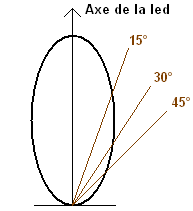
\includegraphics[width=4cm]{ressources/tp1/demi_angle.png}
      \caption{Schéma des différents demis-angles d'une LED}
\end{figure}

\subsection{Objectif et mise au point}

La troisième simulation contient deux lentilles, dont une mobile, par laquelle passe des rayons lumineux.\newline

Sans modifier la position de la source lumineuse, l'image devient nette quand la position $x$ de la lentille mobile 
atteint 4,19. A ce moment, les rayons sont concourants sur le capteur.\newline

\begin{figure}[H]
      \center
      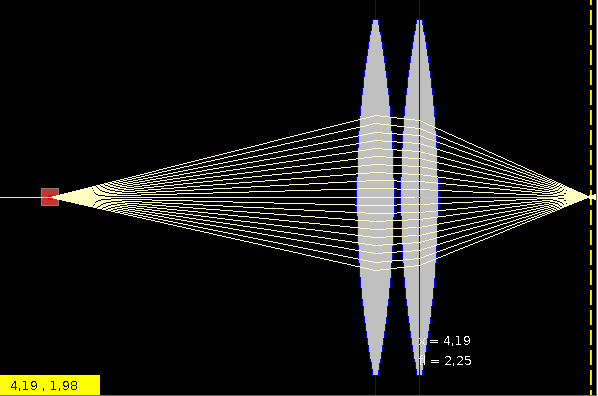
\includegraphics[width=10cm]{ressources/tp1/mise_au_point1.png}
      \caption{Illustration de la mise au point}
\end{figure}

En modifiant la position de la source lumineuse, on peut voir que l'image reste nette tant que la source 
se déplace sur un axe vertical. En effet, la mise au point dépend de la distance de l'objet par rapport à 
l'objectif. Si l'on bouge l'objet sur un axe horizontal, la distance entre l'objet et l'objectif change 
et donc l'image de l'objet n'est plus nette. Il faut alors bouger la lentille mobile pour faire la mise au point. 
On remarque que quand on approche l'objet de l'objectif, à partir d'un certain point l'image de l'objet 
devient virtuelle.\newline

Pour obtenir la distance minimale entre l'objet et l'objectif, il faut coller la lentille mobile à la lentille 
fixe.\newline

Lorsque la source lumineuse est placée à l'infini, on voit que la lentille mobile doit se situer très près du capteur
pour avoir une image nette. En effet, il a été vu précédemment que plus la source lumineuse était proche, plus 
il faut que la lentille mobile soit proche de la lentille fixe. Ici, c'est le contraire.\newline

La distance focale est la distance entre le centre optique de la lentille et son foyer. Quand l'objet se situe à l'infini, 
le foyer est confondu avec la surface du capteur, la distance focale $f$ est donc égale à la distance de 
l'image $b$.\newline


\subsection{Diaphragme et profondeur de champ}

Lorsque la mise au point est correctement effectuée sur l'objet et qu'on change l'ouverture du diaphragme, 
la mise au point reste correcte sur l'objet, les rayons lumineux convergent toujours sur la surface du capteur. 
En effet, la distance objet et la distance focale ne change pas, donc la distance image ne change pas non plus.\newline

Par mesure, la DMO\footnote{Distance minimale de l'objet} est de 3.5. on voit que les calculs donnent le même 
resultat:

\setlength{\columnseprule}{0.4pt}

  \begin{multicols}{3}
    \begin{flushleft}
      $g = 3.5$\\
      $b = b_{max} = 2.17$\\
      $m = \frac{b}{g} = \frac{2.17}{3.5}$\\
      $f = \frac{b}{1+m}$\\
      $DMO = \frac{f * b_{max}}{b_{max} - f} = 3.5$\\
    \end{flushleft}
  \end{multicols}

\begin{figure}[H]
      \center
      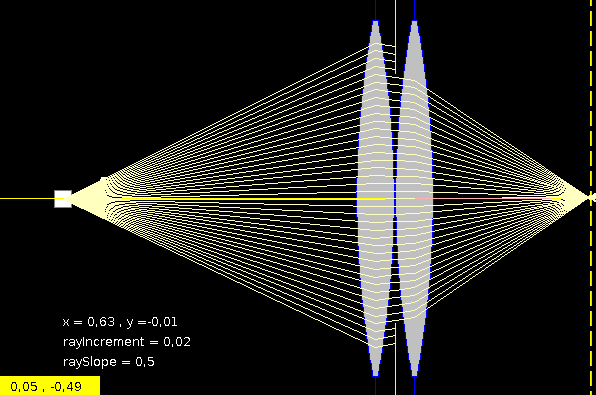
\includegraphics[width=10cm]{ressources/tp1/diaphrage.png}
      \caption{Illustration de la DMO}
\end{figure}

Lorsque l'ouverture du diaphragme est réglée à 0.5 la DMO reste identique, mais la profondeur de champ est 
plus grande, donc moins de flou de profondeur de champ.\newline

Avec une source de lumière à une distance infinie, la lentille de mise au point doit forcément être au plus proche du capteur.
Le diaphragme garde le même effet de limiter la quantité de lumière entrante en réduisant l'ouverture. L'image apparaîtra donc plus sombre avec 
légèrement moins de flou de profondeur de champ.\newline


